%!TEX root = main.tex

\section{Results}
\label{sec:results}

\begin{table*}[tp] \centering
	\begin{minipage}[b]{0.35\textwidth} \centering
		\caption{Resource utilization of design and submodules.}
		\label{tab:results_resource_utilization}
		\begin{tabular}{l r r r r}
			\toprule
							   &    LUT    &    FF     &   Slice   &   BRAM    \\
			\midrule
			Overall            &  64.8\% & 13.06\% & 93.29\% & 95.71\% \\
			\midrule
			quad-core          &  2,777  &    720  &    801  &   13    \\
			single core        &    617  &    132  &    197  &    3    \\
			Blowfish core      &    354  &     64  &     71  &    0    \\
			Password Generator &    216  &    205  &     81  &    0    \\
			\bottomrule\\
		\end{tabular}
	\end{minipage}%
	\hspace{1.5cm}
	\begin{minipage}[b]{0.5\textwidth} \centering
		\caption{Comparison of multiple implementations and platforms, considering
		full system power consumption.}
		\label{tab:results_different_plattforms}
		\begin{tabular}{l c c c c c c}
			\toprule
			& \multicolumn{2}{c}{cost parameter 5}
			& \multicolumn{2}{c}{cost parameter 12}
			& & \\
			& $\frac{\text{Hashes}}{\text{Second}}$
			& $\frac{\text{Hashes}}{\text{Watt Second}}$
			& $\frac{\text{Hashes}}{\text{Second}}$
			& $\frac{\text{Hashes}}{\text{Watt Second}}$
			& Power & Price \\
			\midrule
			zedboard     &  6,511 & 1,550 &  51.95 & 12.37 & \SI{4.2}{\watt} &   \$319 \\
			Virtex-7     & 51,437 & 2,572 & 410.4  & 20.52 & \SI{ 20}{\watt} & \$3,495 \\
			\midrule
			Xeon E3-1240 &  6,210 &  20.7 &  50    &  0.17 & \SI{300}{\watt} &   \$262 \\
			GTX 750 Ti   &  1,920 &   6.4 &  15    &  0.05 & \SI{300}{\watt} &   \$120 \\
			\midrule
			\cite{WOOT/Malvoni14}~Epiphany 16 &  1,207 & 132.64 &  9.64 & 1.06 & \SI{9.1}{\watt} &   \$149 \\
			\cite{WOOT/Malvoni14}~zedboard    &  4,571 & 682.24 & 64.83 & 9.68 & \SI{6.7}{\watt} &   \$319 \\
			\bottomrule\\
		\end{tabular}
	\end{minipage}%
\end{table*}

In this section we will present the results of our implementation. We used
Xilinx ISE 14.7 and -- if needed Xilinx Vivado 2014.1 -- during the design flow
and verified the design both in simulation and on the zedboard after Place and
Route.

Table~\ref{tab:results_resource_utilization} provides the post place-and-route
results of the full design on the zedboard. We implemented the design using ten
parallel bcrypt quad-cores and a Xillybus interface. The design achieves a clock
frequency of 100 MHz. The optimizations from Section~\ref{sec:implementation}
reduced the LUT consumption to roughly 600 LUTs, the amount of BRAMs to 3.25
per single core. We therefore can fit ten quad-cores -- and thus 40 single cores
-- on a zedboard, including the on-chip password generation.

The bcrypt cores need constant cycles $c$ for hash generation, in detail:
\begin{equation*}
\begin{aligned}[c]
c_\text{Reset} &= 1\\
c_\text{Delay} &= 19\\
c_\text{bf} &= 18\\
c_\text{key xor} &= 19\\
\end{aligned}
%\quad
%\begin{aligned}[c]
%\end{aligned}
\quad
\begin{aligned}[c]
c_\text{Init} &= 256\\
c_\text{Pipeline} &= n,\, (n = 2)\\
c_\text{updateP} &= 9 \cdot (c_\text{bf})\\
c_\text{updateSBox} &= 512 \cdot (c_\text{bf})\\
\end{aligned}
\end{equation*}
\begin{align*}
c_\text{ExpandKey} &= c_\text{key xor} + c_\text{upP} + c_\text{upSBox} = 9,397\\
c_\text{EncryptECB} &= 3 \cdot 64 \cdot (c_\text{bf} - 1) = 3,264
\end{align*}
Following these values, one bcrypt hashing needs
\begin{align*}
c_\text{bcrypt} &= c_\text{Reset} + c_\text{Pipeline} + c_\text{Init} +
				   c_\text{Delay} +\\
				&\quad (1 + 2^{\text{cost}+1} \cdot c_\text{ExpandKey}) +
				   c_\text{EncryptECB}\\
				&= 12,939 + 2^{\text{cost}+1} \cdot 9,397
\end{align*}
cycles to finish. This leads to a total of 614,347 cycles per password (cost
5) and 76,993,163 (cost 12), respectively.

In order to compare the design with other architectures, especially with the
previous results on the zedboard, we measured the power consumption of the board
during a running attack and used (ocl)Hashcat to benchmark a Xeon E3-1240 CPU (4
cores@3.1 GHz) and a GTX 750 Ti (Maxwell architecture) as representatives for
the classes of CPUs and GPUs. Furthermore, we synthesized our quad-core
architecture on the Virtex 7 XC7VX485T FPGA, which is available on the VC707
development board, and estimated the number of available cores with respect to
the area a new interface may occupy. We assume a worst-case upper bound of 20W
as the power consumption for the full evaluation board.
For the CPU and the GPU attack, we also consider the complete system. While
there are smaller power supplies available, we consider a 300W power supply,
which is the recommended minimum for the GPU to run stable.

\begin{figure}[tp]
	\centering
	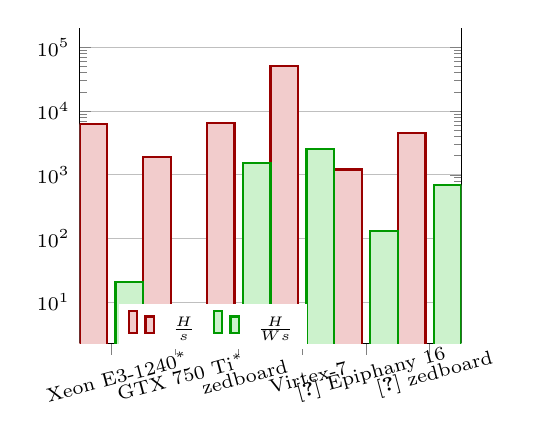
\begin{tikzpicture}[color/.style={draw=#1!80!black,fill=#1!20}]
	\pgfplotsset{
		height=4cm, width=.4\textwidth,
		scale only axis,
		legend style={draw=none,legend cell align=left}}
	\begin{axis}[
		axis x line*=bottom,
		x tick label style={rotate=15,anchor=south,yshift=-5mm,font=\scriptsize},
		y tick label style={font=\scriptsize},
		xtick={1, 2, 3, 4, 5, 6},
		xticklabels={
			Xeon E3-1240$^*$,
			GTX 750 Ti$^*$,
			zedboard,
			Virtex-7,
			\cite{WOOT/Malvoni14}~Epiphany 16,
			\cite{WOOT/Malvoni14}~zedboard},
		xmin=0.5, xmax=6.5,
		ymin=0, ymax=200000,
		ymode=log,
		ymajorgrids=true,
		ybar=3pt,
		bar width=10pt,
		]
		\addplot+[color=red!75!black] plot coordinates{
			(1, 6210)
			(2, 1920)
			(3, 6511)
			(4, 51437)
			(5, 1207)
			(6, 4571)};
		\addplot+[color=green!75!black] plot coordinates{
			(1, 20.7)
			(2, 6.4)
			(3, 1550)
			(4, 2572)
			(5, 132.64)
			(6, 682.24)};
		\legend{$\frac{\text{H}}{\text{s}}$,$\frac{\text{H}}{\text{Ws}}$}
	\end{axis}
	\end{tikzpicture}
	\caption{Comparison of different implementations for cost parameter 5. Left bars
	(red) show the hashes-per-seconds rate, right bars (green) the
	hashes-per-watt-seconds rate. Results with $^*$ were measured with
	(ocl)Hashcat. The axial scale is logarithmic.}
	\label{fig:implementation_comparison}
\end{figure}

\begin{figure*}[tp] \centering
	\hspace{-.5cm}
	\begin{minipage}[b]{0.45\textwidth} \centering
	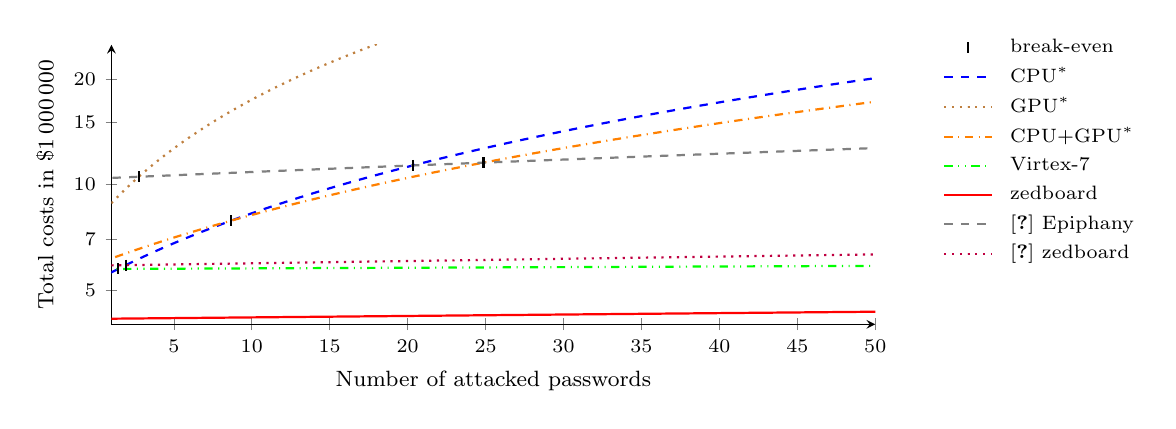
\begin{tikzpicture}
	\pgfplotsset{
		height=3.55cm, width=.8\textwidth,
		scale only axis,
		legend columns=1,
		legend style={at={(1,0.5)},
					  xshift=0.25cm,
					  yshift=1.5cm,
					  anchor=north west,
					  nodes=right,
					  font=\scriptsize,
					 },
		every axis plot post/.append style={
			mark=none,
			domain=0:50,
			samples=100,
			thick},
		}
	\begin{axis}[
		scatter/classes={a={mark=|,black}},
		axis y line=left,
		axis x line=bottom,
		x tick label style={font=\scriptsize},
		y tick label style={font=\scriptsize},
		xlabel style={font=\footnotesize},
		xlabel=Number of attacked passwords,
		ylabel style={font=\footnotesize},
		ylabel=Total costs in \$1\,000\,000,
		%xtick={25, 50, 75, 100, 125, 150, 175},
		xmin=1, xmax=50,
		ytick={5000000, 7000000, 10000000, 15000000, 20000000},
		yticklabels={$5$, $7$, $10$, $15$, $20$},
		ymin=4000000, ymax=25000000,
		ymode=log,
		cycle list name=linestyles*
		]
		\addplot+[color=black,only marks,scatter,scatter src=explicit symbolic] coordinates{
			(2.75, 10525390.42) [a]
			(1.91, 5895676.33) [a]
			(20.33, 11335789.16) [a]
			(1.43, 5752687.56) [a]
			(24.86, 11544263.66) [a]
			(8.69, 7897759.68) [a]
			(1017.0, 8177871.0) [a]
		};
		\addplot+[color=blue]{5330652+295327*x}; %CPU
		\addplot+[color=brown]{7896960+955217*x}; %GPU
		\addplot+[color=orange]{5936853+225588*x}; %CPU+GPU
		\addplot+[color=green]{5749275+2388*x}; %Virtex7
		\addplot+[color=red]{4146681+3963*x}; %zedboard
		\addplot+[color=gray]{10398561+46092*x}; %Epiphany
		\addplot+[color=purple]{5878532+8961*x}; %OWzb
		\legend{
			break-even, CPU$^*$, GPU$^*$, CPU+GPU$^*$,
			Virtex-7, zedboard,
			\cite{WOOT/Malvoni14}~Epiphany, \cite{WOOT/Malvoni14}~zedboard
			}
	\end{axis}
	\end{tikzpicture}
	\caption{Total costs in \textit{millions USD} for attacking $n$ passwords of length 8 from a set of
	62 characters, with logarithmic scale. Each attack finishes within
	\textit{one month}. Both the acquisition costs for enough devices and the total power costs
	where considered.}
	\label{fig:costs_for_password_cracking}
	\end{minipage}%
	\hspace{2.cm}
	\begin{minipage}[b]{0.45\textwidth} \centering
	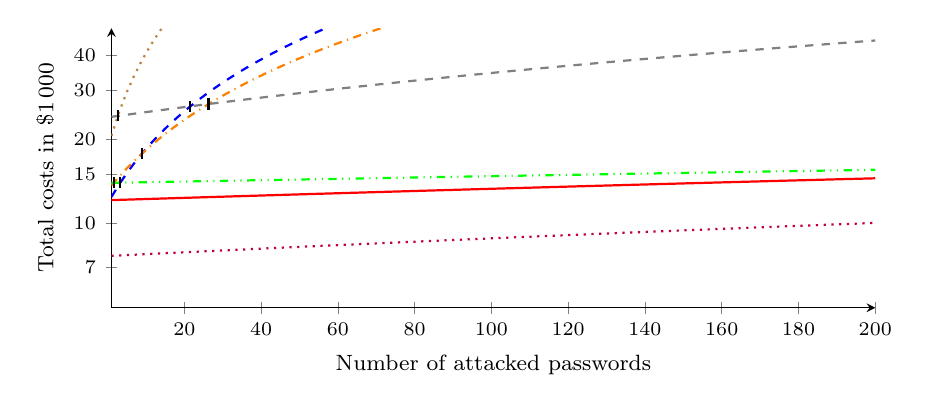
\begin{tikzpicture}
	\pgfplotsset{
		height=3.55cm, width=.8\textwidth,
		scale only axis,
		legend columns=3,
		legend style={column sep=1ex,
					  at={(0,0)},
					  xshift=0.25cm,
					  yshift=-1.0cm,
					  anchor=north west,
					  nodes=right,
					  font=\scriptsize
					 },
		every axis plot post/.append style={
			mark=none,
			domain=1:200,
			samples=100,
			thick},
		}
	\begin{axis}[
		scatter/classes={a={mark=|,black}},
		axis y line=left,
		axis x line=bottom,
		x tick label style={font=\scriptsize},
		y tick label style={font=\scriptsize},
		xlabel style={font=\footnotesize},
		xlabel=Number of attacked passwords,
		ylabel style={font=\footnotesize},
		ylabel=Total costs in \$1\,000,
		%xtick={25, 50, 75, 100, 125, 150, 175},
		xmin=1, xmax=200,
		ytick={7000, 10000, 15000, 20000, 30000, 40000},
		yticklabels={$7$, $10$, $15$, $20$, $30$, $40$},
		ymin=5000, ymax=50000,
		ymode=log,
		cycle list name=linestyles*
		]
		\addplot+[color=black,only marks,scatter,scatter src=explicit symbolic] coordinates{
			(0.5, 12128.04) [a]
			(1.57, 13992.59) [a]
			(26.3, 26776.98) [a]
			(2.64, 24268.6) [a]
			(1581.0, 26628.0) [a]
			(464.0, 17692.0) [a]
			(21.55, 26273.62) [a]
			(3.3, 14006.39) [a]
			(8.96, 17811.99) [a]
		};
		\addplot+[color=blue]{11790+672*x}; % CPU
		\addplot+[color=brown]{18360+2240*x}; % GPU
		\addplot+[color=orange]{13179+517*x}; % CPU+GPU
		\addplot+[color=green]{13980+8*x}; % Virtex7
		\addplot+[color=red]{12122+12*x}; % zedboard
		\addplot+[color=gray]{23989+106*x}; % Epiphany
		\addplot+[color=purple]{7656+12*x}; % OWzb
	\end{axis}
	\end{tikzpicture}
	\caption{Total costs in \textit{thousands USD} for attacking $n$ passwords of length 8 from a set of
	62 characters using a cost parameter of 12 (which is commonly recommended),
	with logarithmic scale. Each attack finishes within \textit{one day}, with a
	\textit{dictionary attack} where 65\% are covered ($\text{4} \cdot \text{10}^\text{9}$ Tests).}
	\label{fig:costs_for_dict_attack}
	\end{minipage}%
\end{figure*}

Table~\ref{tab:results_different_plattforms} compares the different
implementation platforms for cost parameter of 5 and 12. For better
comparison, Figure~\ref{fig:implementation_comparison} shows the performance and
efficiency graphically only for the first case.
%
Our zedboard implementation outperforms the previous implementation from
\cite{WOOT/Malvoni14} by a factor of 1.42, computing 6511~pps at a measured
power consumption of only 4.2W compared to 6.7W of the previous
implementation. Thus, this implementation yields also a better power efficiency
of 1550 pps per watt, which is more than twice as efficient as the previous
implementation. The CPU attack on a Xeon computes 5\% less pps, at a
significantly higher power consumption. Even considering only the power
consumption of the CPU itself of 80W, the efficiency of the zedboard is still
about 20 times higher. The estimated Virtex-7 design shows that the
high-performance board is a decent alternative to the zedboard: it outperforms
all other platforms with 51437 pps and has a very high power-efficiency rating.
The drawback is the high price of \$3495 for the development board.

To analyze the full costs of an attack, including the necessary power
consumption (at the price of 10.08 cents per kWh\footnote{Taken from the
\enquote{Independent Statistics \& Analysis U.S. Energy Information
Administration}, average retail price of electricity United States all sectors.
\url{http://www.eia.gov/electricity/data/browser}}), we consider two different
scenarios. The first uses the fairly low cost parameter of 5 for a simple
brute-force attack on passwords of length 8 with 62 different characters and
requires the runtime to be at most 1 month. We chose the considerably low cost
parameter for comparison with the related work, as it is typically used for
bcrypt benchmarks. However, this value is insecure for practical
applications, where a common choice seems to be 12, which is also used in
the related work. Thus, we use this more reasonable parameter in the second setting.
Here, the adversary uses more sophisticated attacks and aims for a reduction of
the number of necessary password guesses and for a reduced runtime of one day
per cracked password: We consider an adversary with access to meaningful,
target-specific, custom dictionaries -- for example generated through social
engineering -- and derivation rules.
%
In~\cite{PBKDEvalutation}, the authors trained on a random subset of 90\% from
the leaked RockYou passwords to attack the remaining 10\% and estimated that
$\text{4} \cdot \text{10}^\text{9}$ guesses are needed for about 67\% chance of
success, which we use as a basis for the computational power.

Figure~\ref{fig:costs_for_password_cracking} shows the costs of running
brute-force attacks in the first scenario. To achieve the requested amount of
password tests in one month, we need 13564 single CPUs, 43872 GPUs,
10361 CPUs + GPUs, 12999 zedboards or 1645 Virtex-7 boards. The figure
shows the total costs considering acquisition costs (fixed cost) and the power
consumption. It reveals the infeasibility of CPUs for attacking password hashes,
and even more clearly the efficiency of special-purpose devices. Even
high-performance FPGAs like the Virtex-7 are more profitable after only a few
password cracks, than a combination of CPU and GPU.

Figure~\ref{fig:costs_for_dict_attack} shows the costs of attacking multiple
passwords in the second scenario. Here, we need 30 CPUs, 102 GPUs, 23
CPUs + GPUs, 38 zedboards or 4 Virtex-7 boards.
%Even though we consider a much higher cost parameter and require a runtime of
%one day per password, the attack is still cheaper due to the smarter derivation
%of password candidates.
With the higher cost parameter our current zedboard implementation does not yield
similar good results and thus \cite{WOOT/Malvoni14} implementation is currently
better suited for this attack when mounted on a zedboard. With the higher cost
parameter, their implementation can conceal an interface bottleneck coming from
the initialization of the bcrypt cores. As our implementation does not suffer from
this bottleneck, we can run several cores on a bigger FPGA without negative
consequences. Please note that the Virtex-7, after amortizing its acquisition costs,
outperforms every other platform (reaching the break-even point with
\cite{WOOT/Malvoni14} zedboard after attacking about 1500 passwords).

%Comparing CPUs with low-power targets like the zedboard leads to the same result
%as before -- power efficiency has a great impact on overall attack costs.
%Therefore, FPGA platforms are better suited for attacking passwords and a
%successful attacker does not have to spend more than \$10000 for cracking
%passwords.
